\documentclass{article}
\usepackage{amsmath, amssymb, kotex, hyperref, graphicx, mdframed, setspace,enumitem}
\usepackage[a4paper, margin = 40pt]{geometry}
\setstretch{1.5}
\newcommand\ar{\ensuremath{\text{AR}}}
\newcommand\ma{\ensuremath{\text{MA}}}
\newcommand\arma{\ensuremath{\text{ARMA}}}
\newcommand\cov{\ensuremath{\text{Cov}}}
\newcommand\sa{\ensuremath{{\sigma_a}^2}}

\begin{document}
\title{Arima Model - 6}
\author{강의 : 김성범 교수님\\ 정리 :  김선중}
\date{\today}
\maketitle

이것은 \href{https://youtu.be/K7GWJ3iC6OY}{ARIMA 모델 개요 - Part 6} 강의에 대한 노트이다.
이번 내용은 계산이 많으므로, 설명을 길게 쓰는 것보다는 계산을 나열하는 것 위주로 정리했다.
다만, conditional expectation과 prediction interval에 대해서는 조금 공부해야 할 것 같아서 간략하게 적어보있다.
지난 번에는 영어로 적었었는데, 이번에는 다시 한글로 적었다.
\tableofcontents

\newpage
\begin{center}
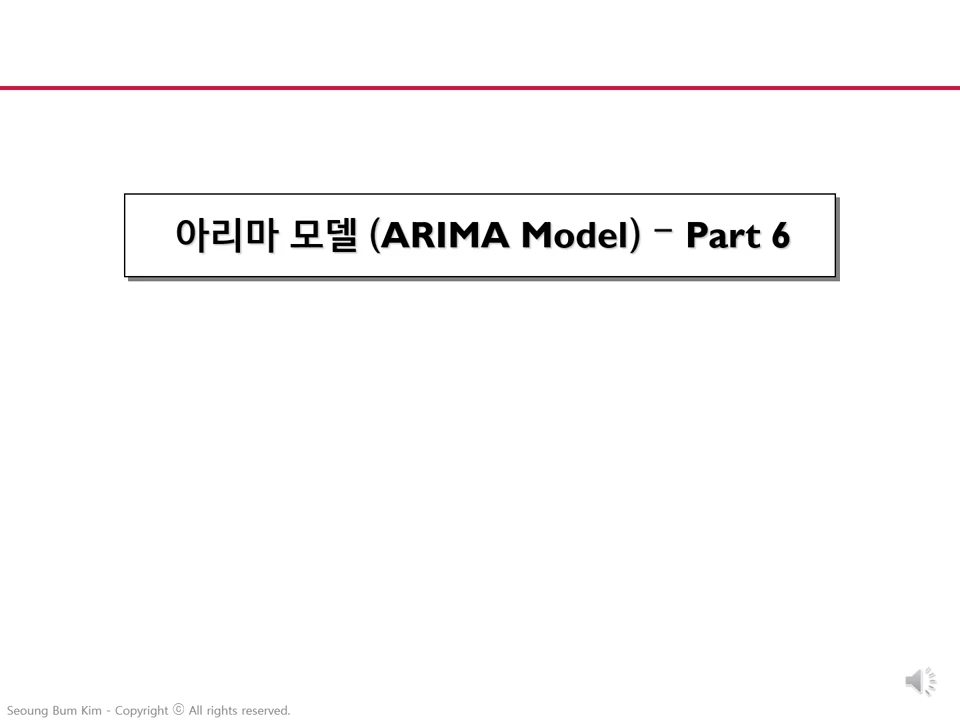
\includegraphics[width=.45\textwidth]{capture_01}
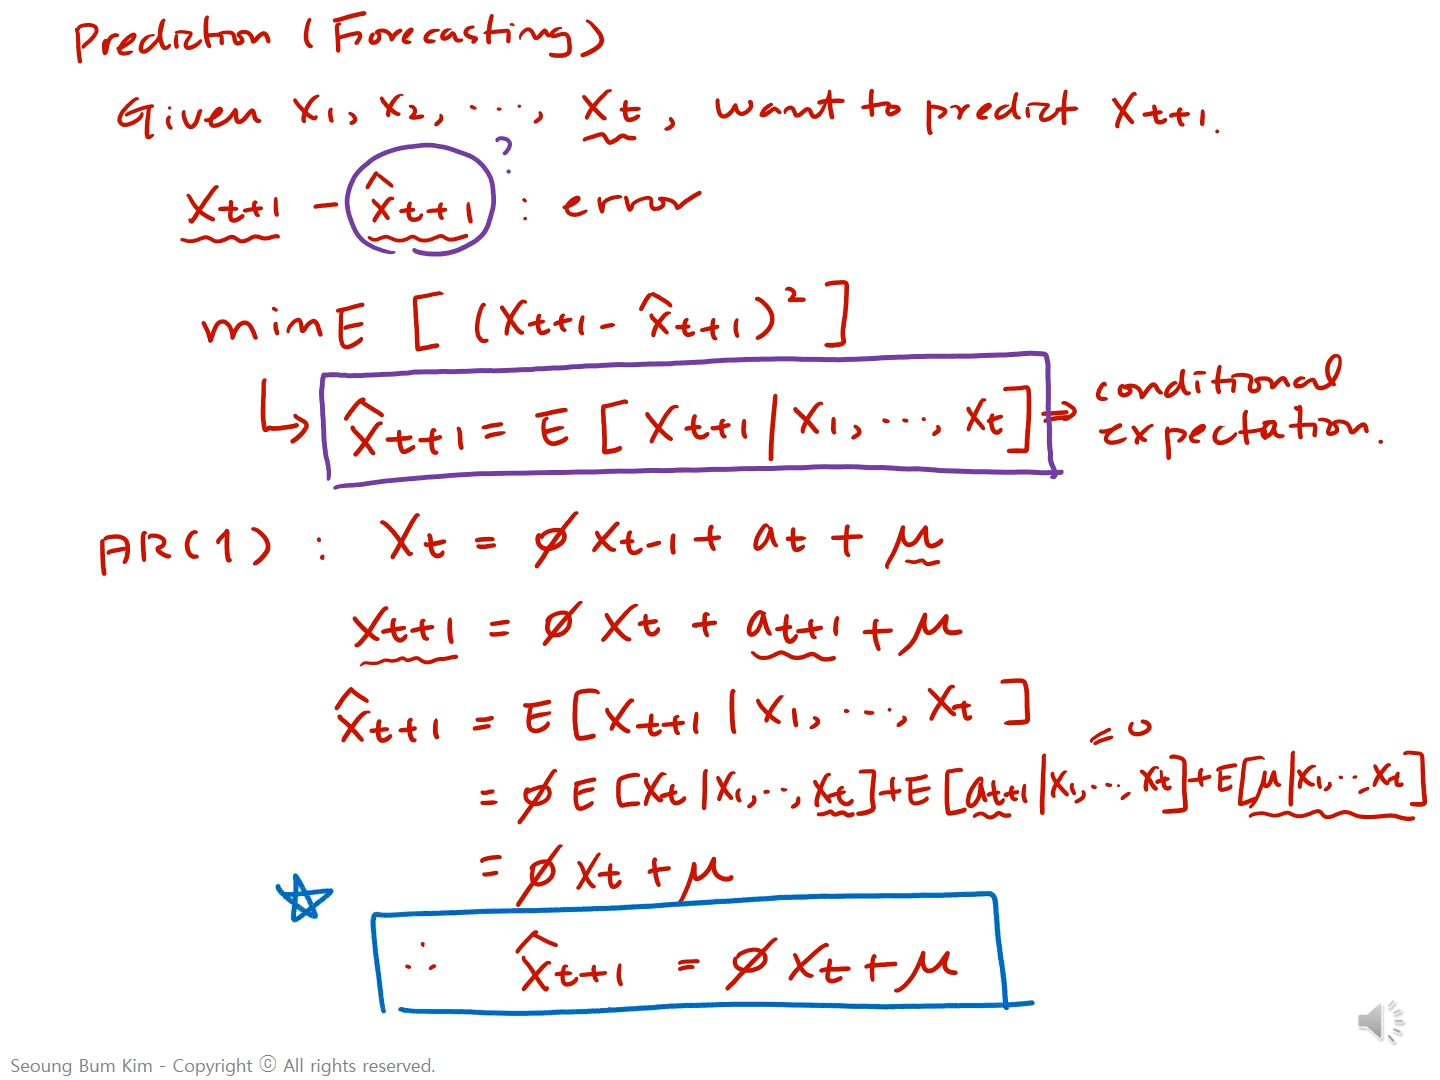
\includegraphics[width=.45\textwidth]{capture_02}
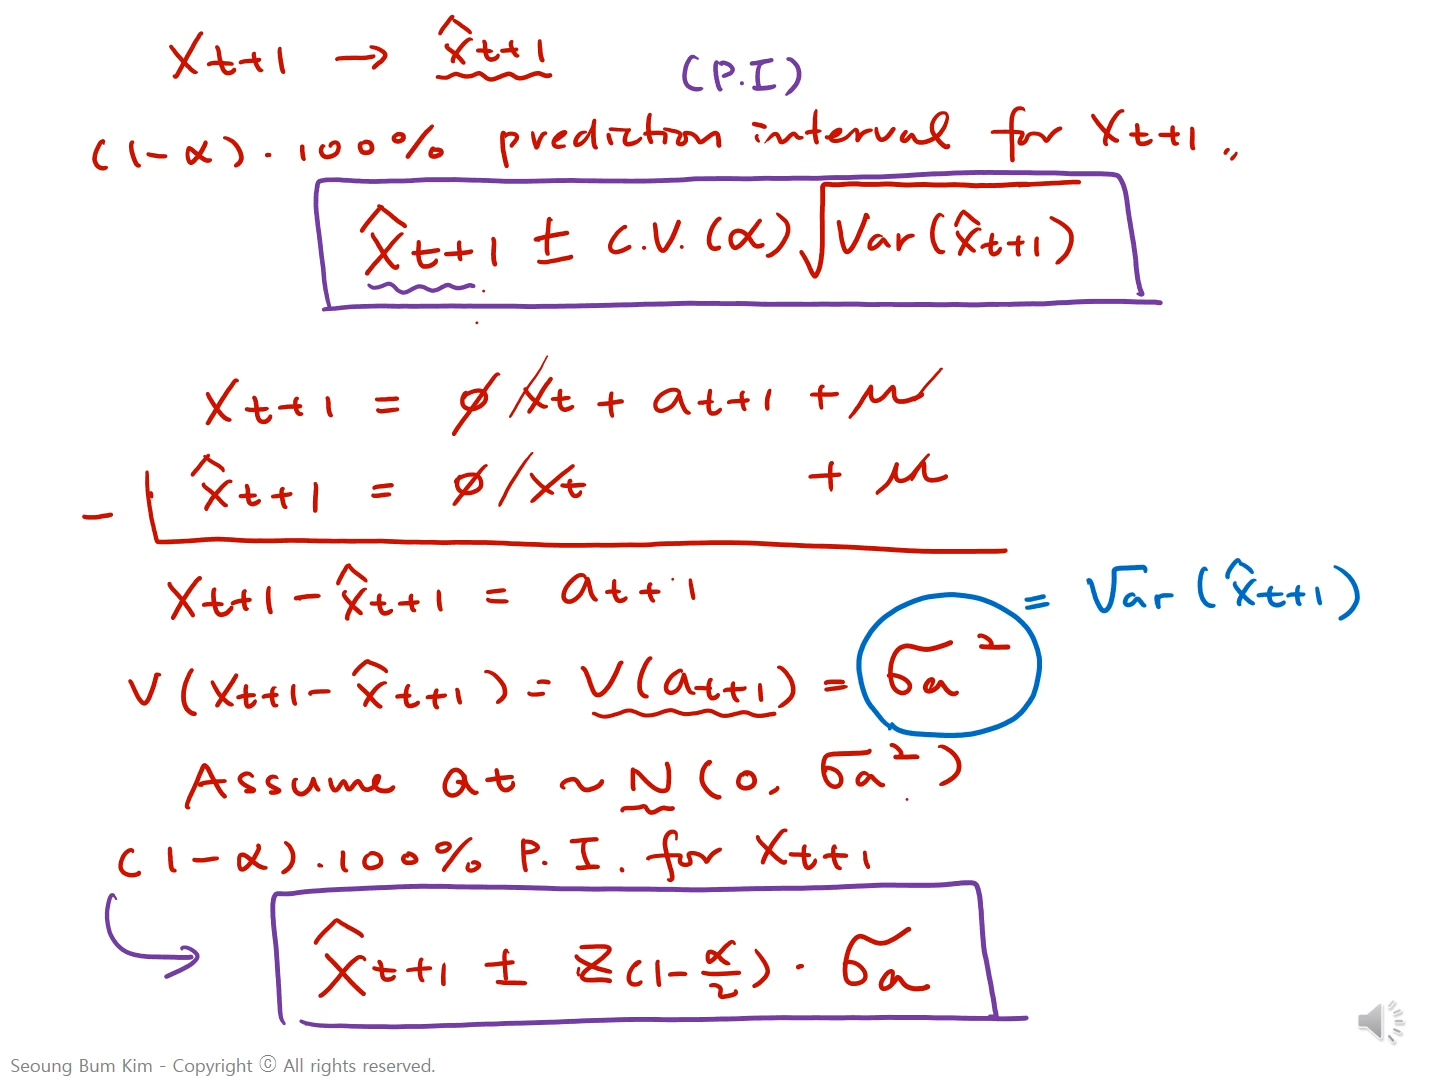
\includegraphics[width=.45\textwidth]{capture_03}
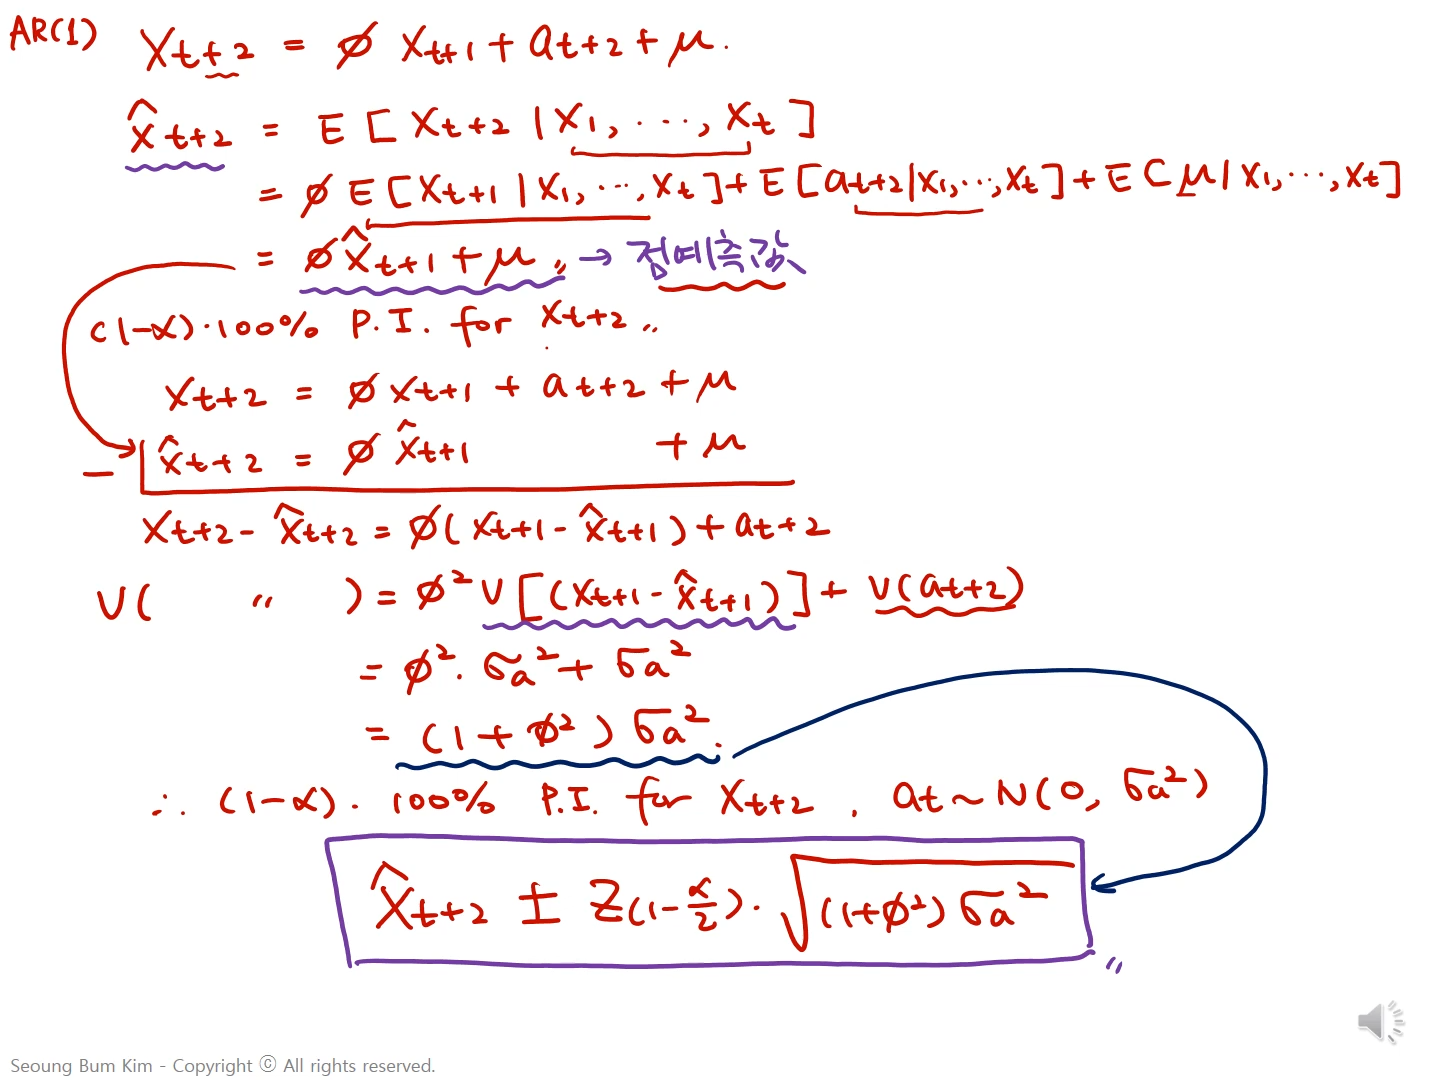
\includegraphics[width=.45\textwidth]{capture_04}
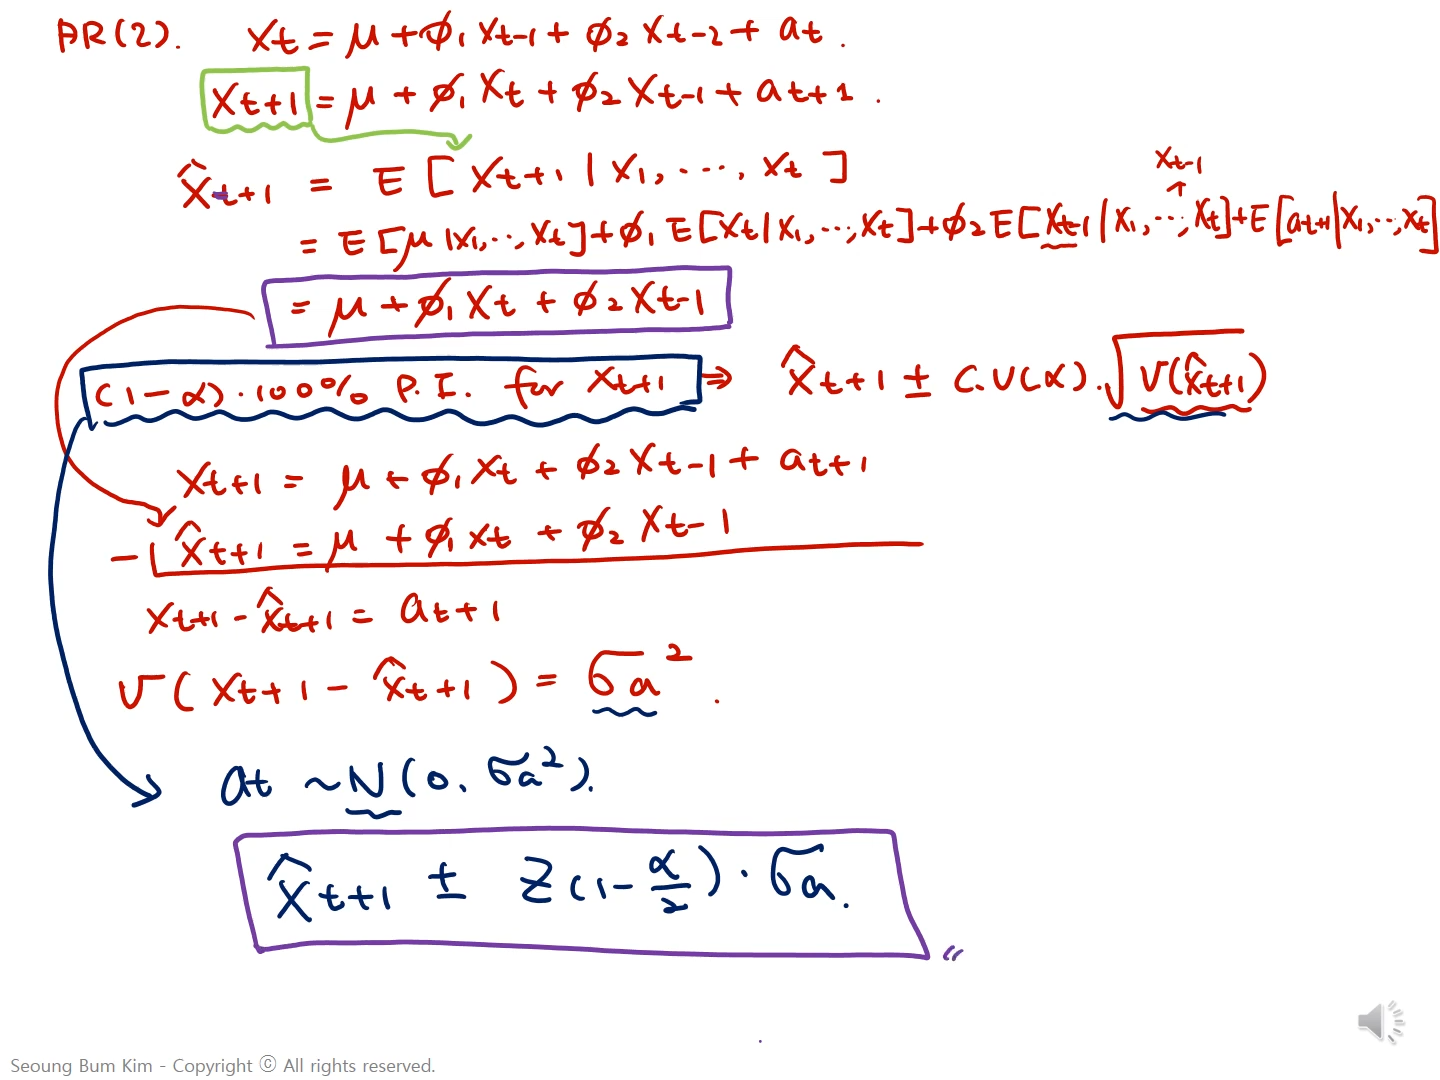
\includegraphics[width=.45\textwidth]{capture_05}
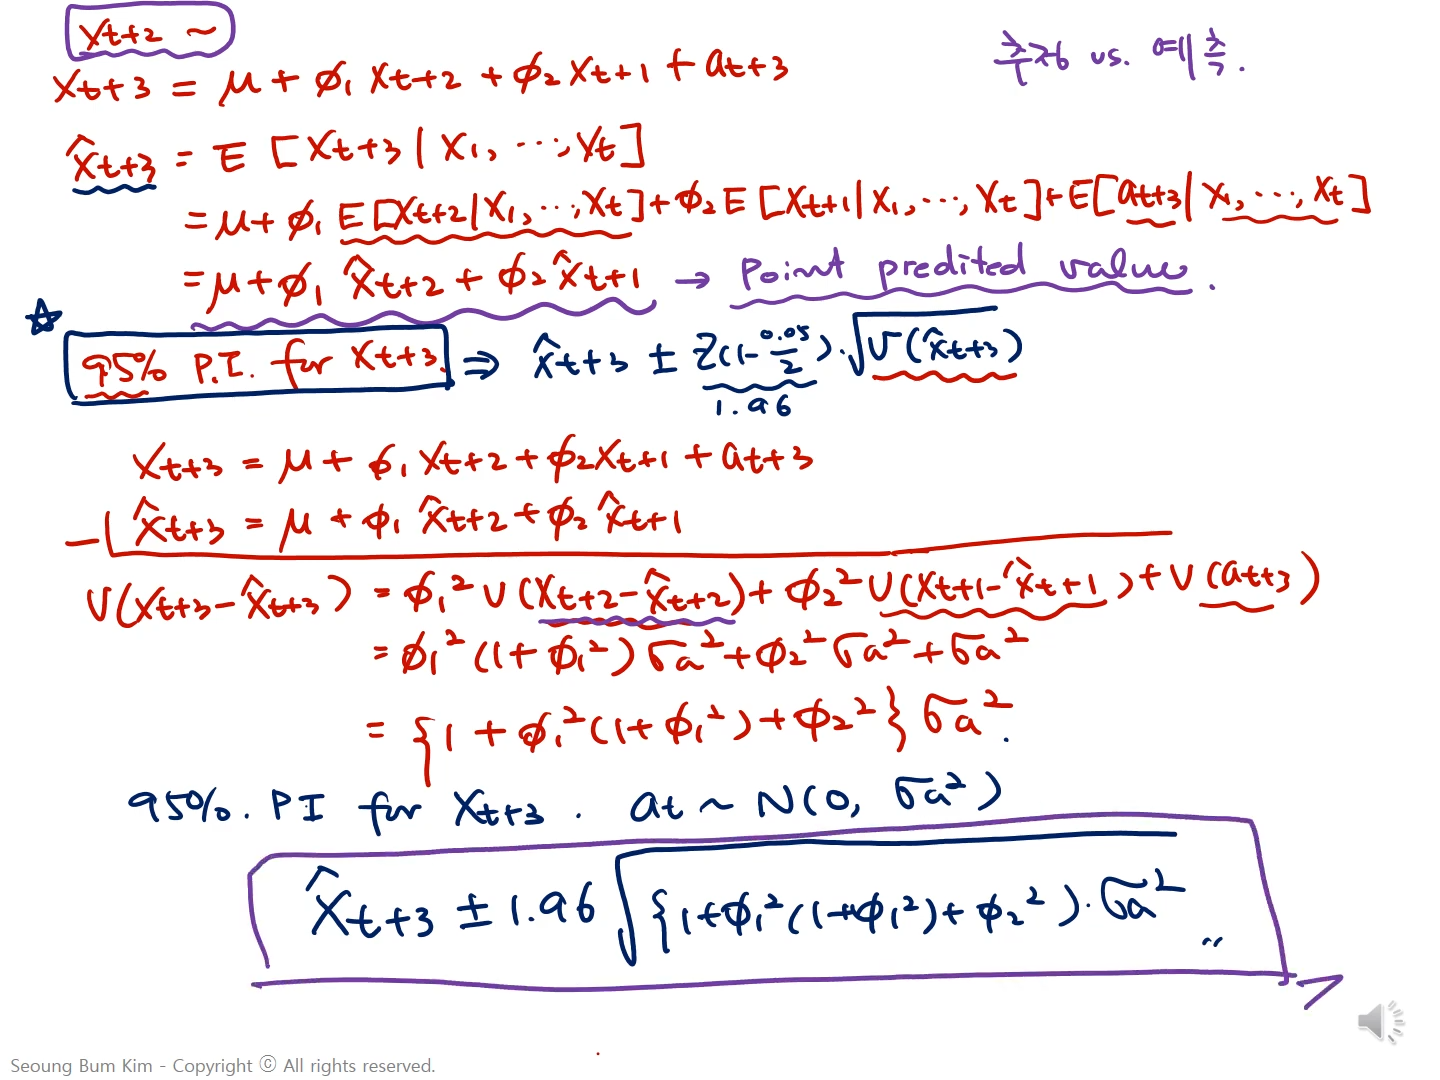
\includegraphics[width=.45\textwidth]{capture_06}
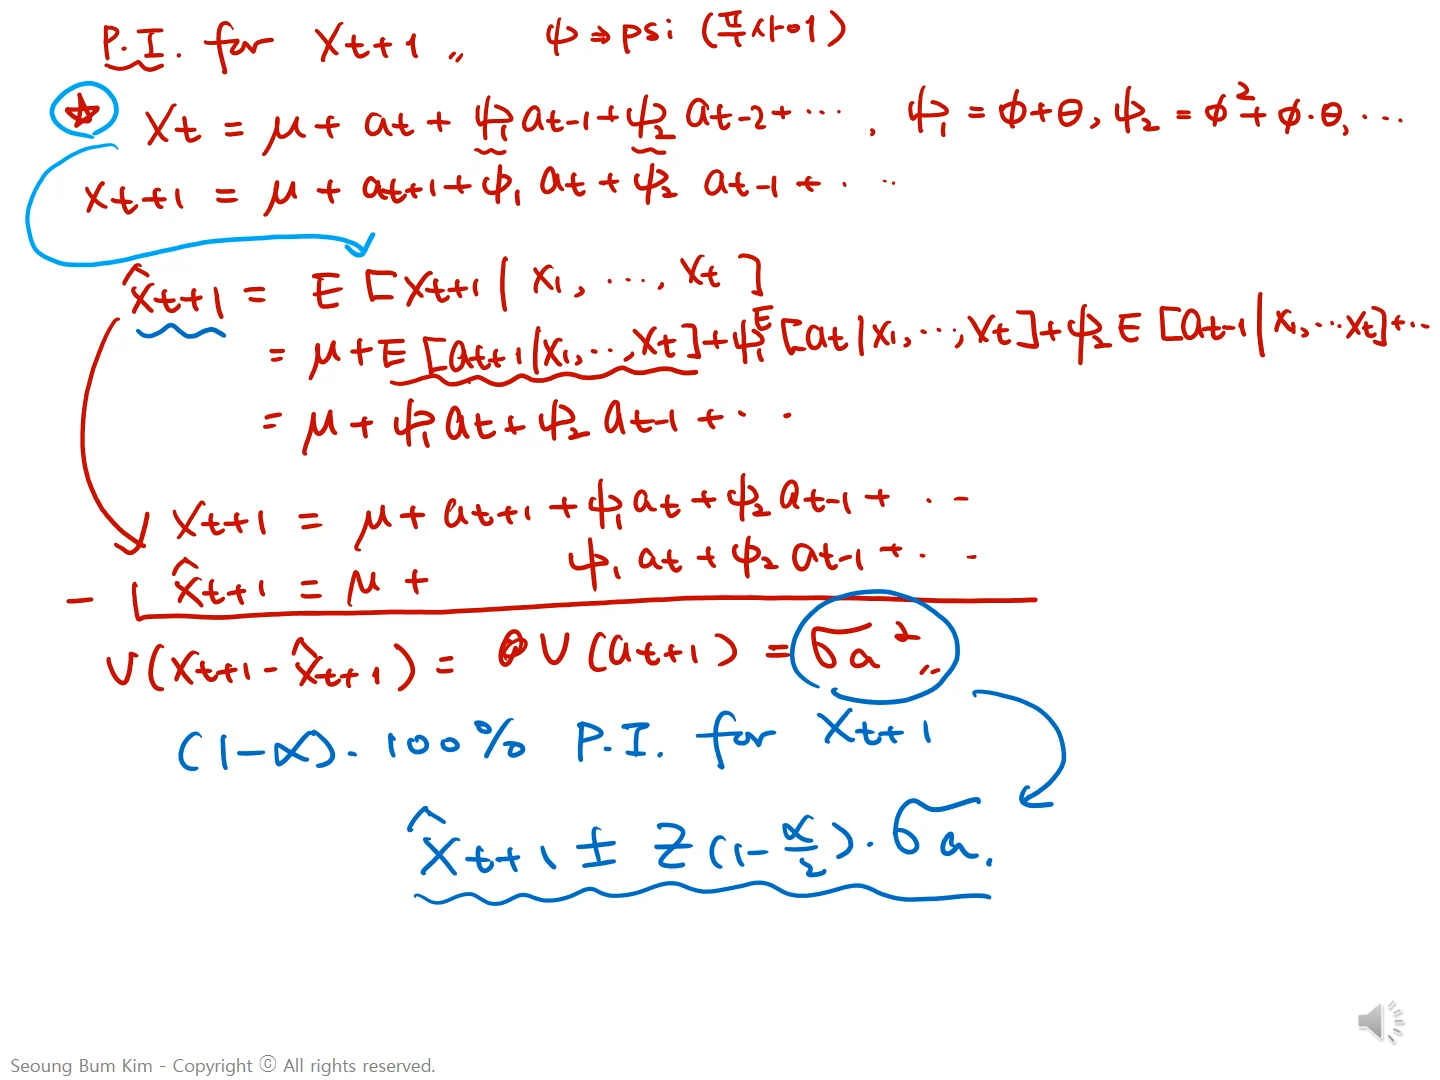
\includegraphics[width=.45\textwidth]{capture_07}
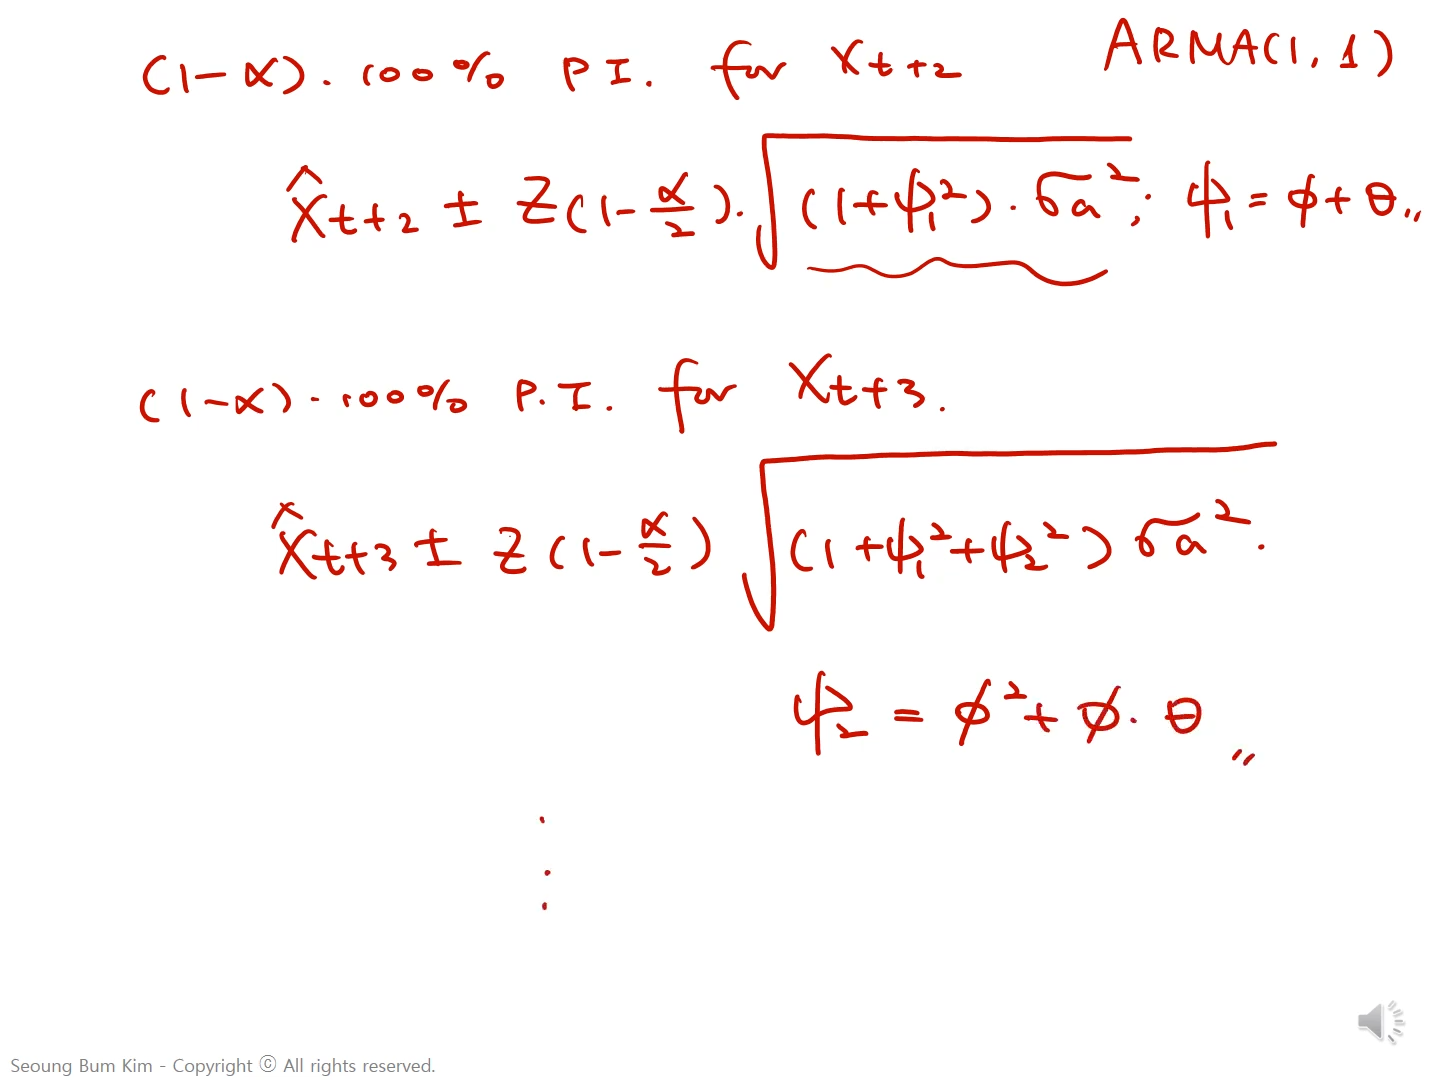
\includegraphics[width=.45\textwidth]{capture_08}
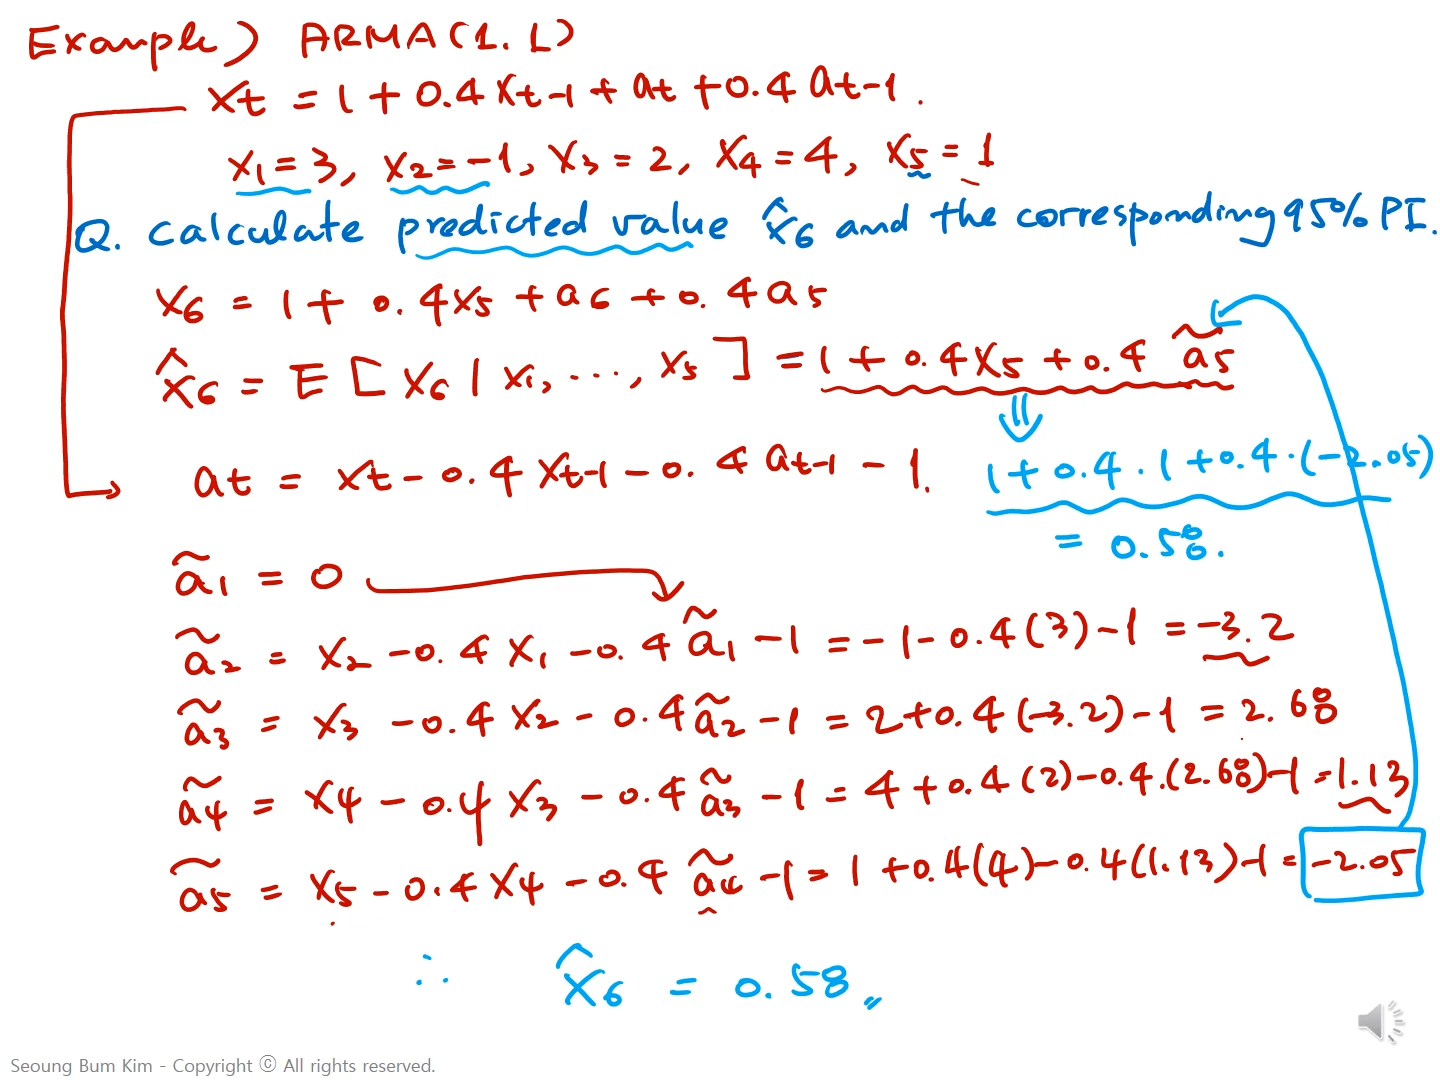
\includegraphics[width=.45\textwidth]{capture_09}
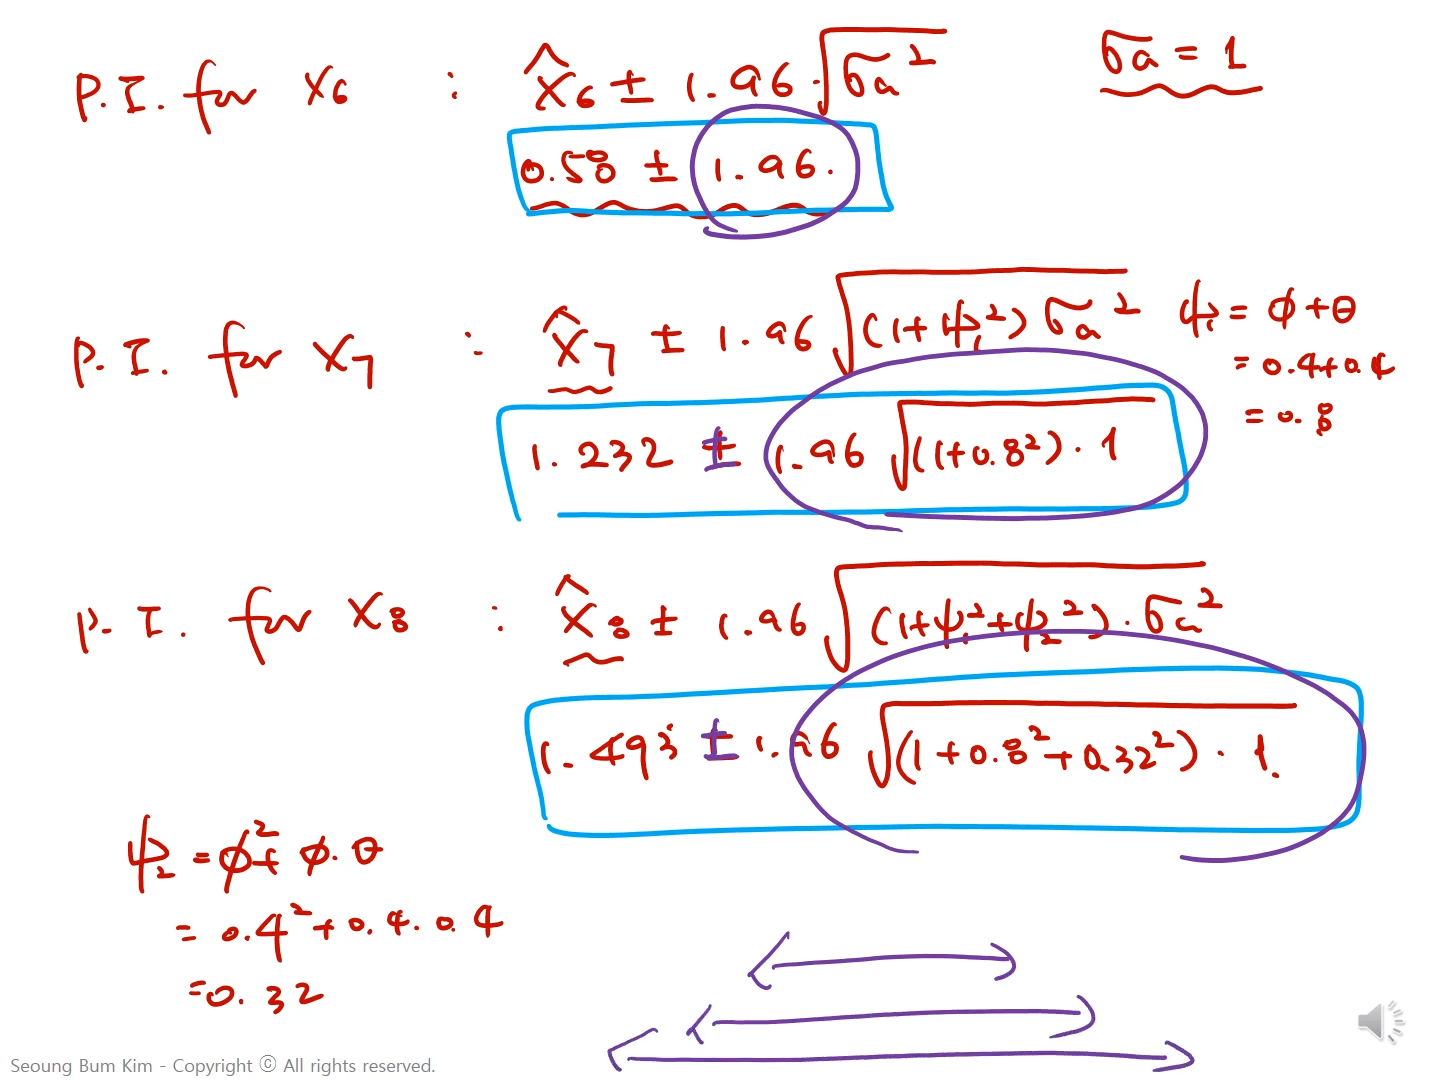
\includegraphics[width=.45\textwidth]{capture_10}
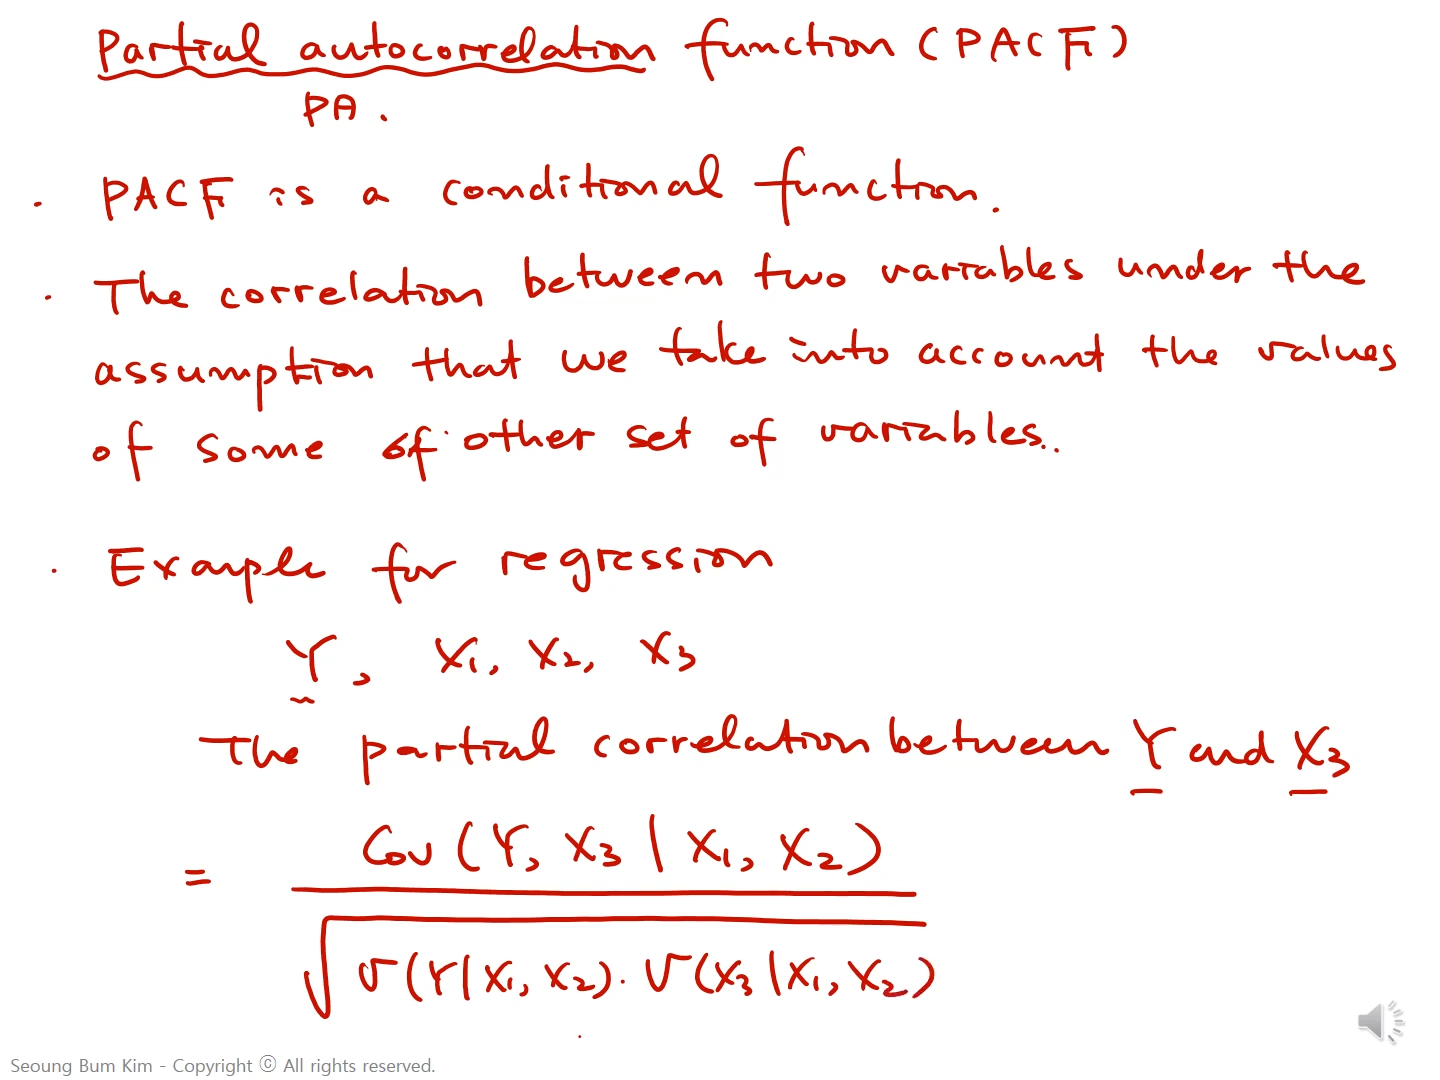
\includegraphics[width=.45\textwidth]{capture_11}
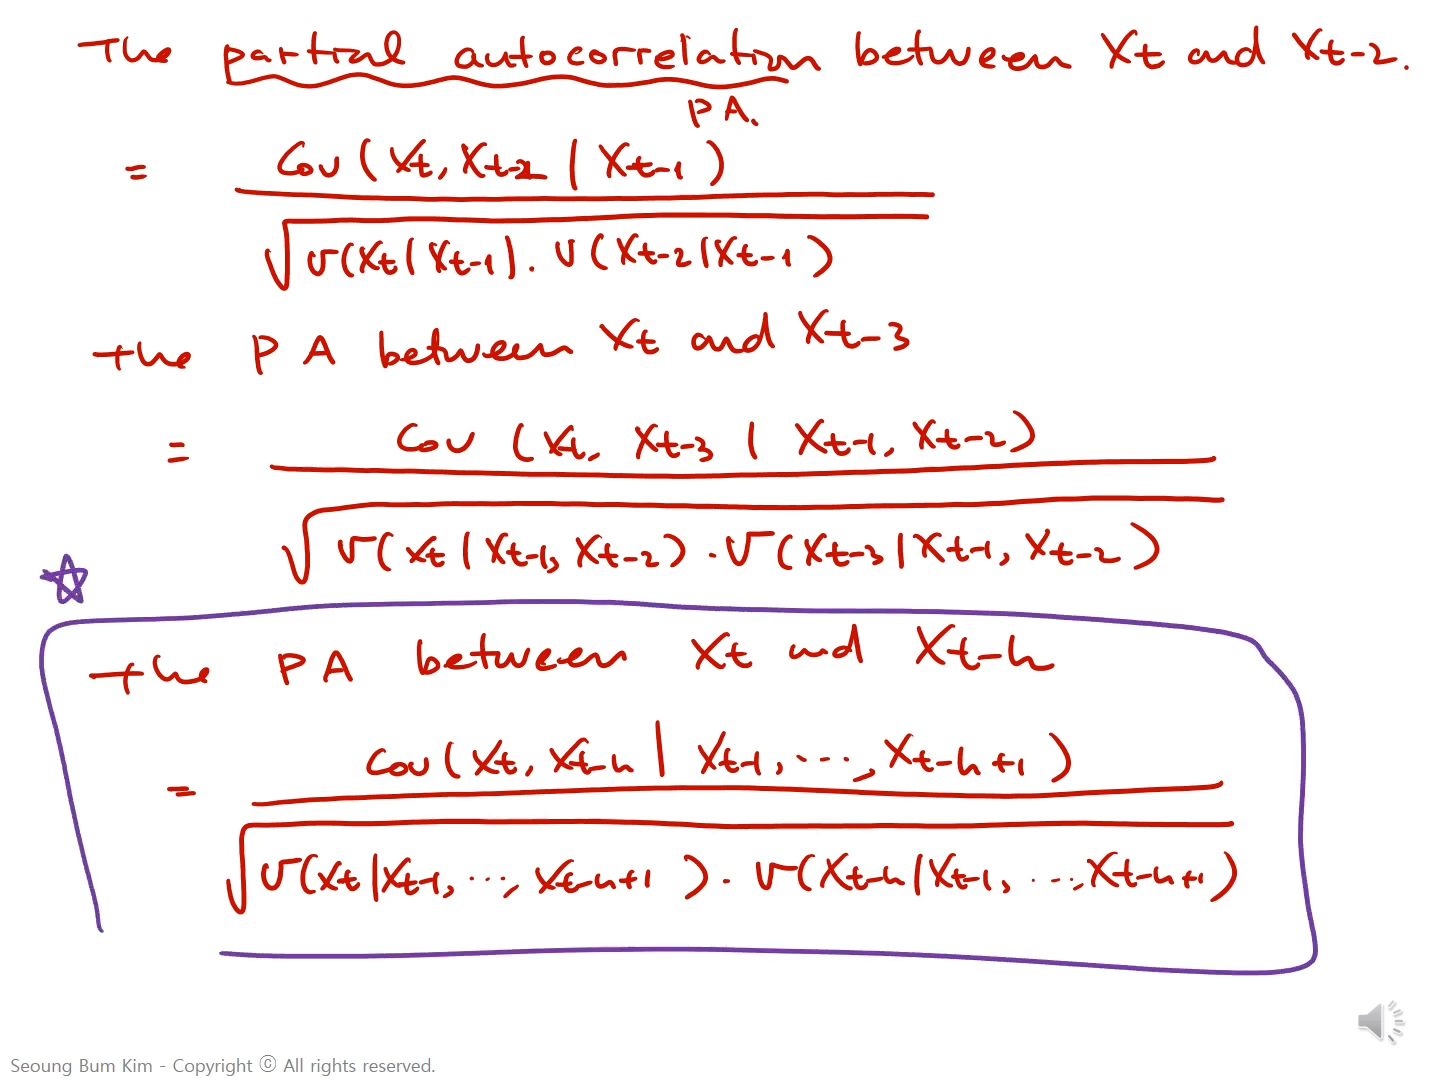
\includegraphics[width=.45\textwidth]{capture_12}
\end{center}

%%%
\section{Preliminaries}

%%
\subsection{Conditional Expectations}

Conditional expectation에 관해서는 \href{https://www.math.arizona.edu/~tgk/464_07/cond_exp.pdf}{이 자료(A Conditional expectation - Arizona Math)}참조했습니다.
해당 자료의 A.1, A.2를 옮겨서 적었습니다.

%
\subsubsection{Probability Spaces}
확률공간 \((\Omega,\mathcal F,\mathbb P)\)을 고려하자.
늘 그렇듯이 \(\Omega\)는 표본공간(sample space)이고, \(\mathcal F\)는 사건공간(event space)이고, \(\mathbb P\)는 확률측도(probability measure)이다.
사건(event)이란, 표본 공간 \(\Omega\)의 부분집합이고, \(\mathcal F\)는 사건들의 집합이지만 모든 사건들의 집합일 필요는 없다. 그보다는, \(\mathcal F\)는 \(\Omega\)에 대한 \(\sigma\)-algebra이라서 세 가지 정도의 성질을 만족시키는 집합이다.
\(\mathbb P\)는 유한측도(finite measure)로서 역시 세가지 정도의 성질을 만족시킨다.

%
\subsubsection{Expectations}
이산확률변수(discrete random variable) \(X\)에 대하여 기댓값(expectation) \(\mathbb E[X]\)은
\[\mathbb E[X]=\sum_xx\mathbb P(X=x)\]
이다.
이때, \(x\mapsto\mathbb P(X=x)\)는 확률질량함수(probability mass function)이다.
연속확률변수(continuous random variable) \(X\)에 대하여는
\[\mathbb E[X]=\int_xxf(x)\,dx\]
와 같은 정의가 있다.
이때에는 \(f(x)\)는 확률밀도함수(probability density function)로서
\[\int_a^bf(x)\,dx=\mathbb P(a\le X\le b)\]를 만족하는 함수이다.

%
\subsubsection{Joint and Marginal Distributions}
두 확률변수 \(X\), \(Y\)에 대하여는 이 확률변수들의 순서쌍 \((X,Y)\)이 하나의 확률변수가 된다.
이 확률변수의 분포를 결합확률분포(joint distribution)라고 한다.
만약 \(X\)와 \(Y\)가 모두 이산확률변수이면, \((X,Y)\) 또한 이산확률변수이고, 이때의 확률질량함수는
\[\mathbb P(X=x, Y=y)\]
와 같은 이변수함수가 된다.
\(X\)와 \(Y\)에 대한 함수 \(g(X,Y)\)가 있을 때, \(g(X,Y)\)에 대한 기댓값 \(\mathbb E[g(X,Y)]\)은
\[\mathbb E[g(X,Y)]=\sum_xg(x,y)\mathbb P(X=x,Y=y)\]
가 된다.
간단한 예로, 확률변수 \(X+3Y\)에 대한 기댓값 \(\mathbb E[X+3Y]\)은 (\(g(X,Y)=X+3Y\))
\[\mathbb E[X+3Y]=\sum_{x,y}(x+3y)\mathbb P(X=x,Y=y)\]
이고, 확률변수 \(X^2Y\)에 대한 기댓값 \(\mathbb E[X^2Y]\)은 (\(g(x,Y)=X^2Y\))
\[\mathbb E[X^2Y]=\sum_xx^2y\mathbb P(X=x,Y=y)\]
이다.
만약 \(X\)와 \(Y\)가 모두 연속확률변수이면 \((X,Y)\) 또한 연속확률변수가 된다.
\(X\)가 연속확률변수라고 할 때에는 \(X:\Omega_X\to\mathbb R\)이라는 의미였지만, \((X,Y)\)가 연속확률변수라고 말할 떄에는 \((X,Y):\Omega_X\times\Omega_Y\to\mathbb R^2\)이라는 의미가 된다.
확률변수 \((X,Y)\)의 확률밀도함수 \(f_{X,Y}\)는
\[\int_a^b\int_c^df_{X,Y}(x,y)\,dx\,dy=\mathbb P(a\le x\le b,c\le x\le d)\]
를 만족시키는 이변수 함수이다.
함수 \(g(X,Y)\)에 대한 기댓값 \(\mathbb E[g(X,Y)]\)는
\[\mathbb E[g(X,Y)]=\iint_{x,y}g(x,y)f_{X,Y}(x,y)\,dx\,dy\]
이다.
위에서와 같은 예를 들어서 설명하면
\begin{align*}
\mathbb E[X+3Y]&=\iint_{x,y}(x+3y)f_{X,Y}(x,y)\,dx\,dy\\
\mathbb E[X^2Y]&=\iint_{x,y}x^2yf_{X,Y}(x,y)\,dx\,dy\\
\end{align*}
이 된다.

결합확률분포의 관점에서 보면 \(X\)의 확률분포(혹은 \(Y\)에 대한 확률분포)는 \((X,Y)\)에 대한 주변확률분포(marginal distribution)이라고 말할 수 있다.
\(X\), \(Y\) 대한 확률질량함수[혹은 확률밀도함수]를 \(X\)에 대하여 (혹은 \(Y\)에 대하여) marginalize하면 \(Y\)(혹은 \(X\))에 대한 확률질량함수 [혹은 확률밀도함수]가 얻어지는 것이다.
이것을 수식으로 쓰면, 이산확률변수에 대해서는
\begin{align*}
\sum_x\mathbb P(X=x,Y=y)&=\mathbb P(Y=y)\\
\sum_y\mathbb P(X=x,Y=y)&=\mathbb P(X=x)
\end{align*}
이 성립하고, 연속확률변수에 대해서는
\begin{align*}
\int_xf_{X,Y}(x,y)&=f_Y(y)\\
\int_yf_{X,Y}(x,y)&=f_X(x)
\end{align*}
이 성립한다는 말이 된다.

여러 개의 확률변수 \(X_1\), \(X_2\), \(\cdots\), \(X_N\)에 대해서도 새로운 확률변수 \((X_1,X_2,\cdots,X_N)\)를 생각할 수 있다.
이것은, 그러니까 확률변수들의 tuple인 것이다.
확률변수 \(X_n\) (\(1\le n\le N\))들이 모두 이산확률변수일 경우, 확률질량함수
\[\mathbb P(X_1=x_1,X_2=x_2,\cdots,X_N=x_N)\]
을 생각할 수 있고, 모두 연속확률변수인 경우, 확률밀도함수
\[f_{X_1,X_2,\cdots,X_N}(x_1,x_2,\cdots,x_N)\]
을 생각하게 된다.\footnote{
그런데 위의 표현은 너무 복잡하므로, 그냥 간단하게
\[f_{\boldsymbol X}(x_1,x_2,\cdots,x_N)\]
라고 쓸 수도 있을 것이다.
즉 \(\boldsymbol X=(X_1,X_2,\cdots,X_N)\)이라고 생각하는 것이다.}
이것들은 당연히 이변수일 때와 비슷한 성질을 만족시킬 것이지만 여기에 적지는 않겠다.
함수 \(g(X_1,X_2,\cdots,X_N)\)에 대한 기댓값은
\[\mathbb E[g(X_1,X_2,\cdots,X_N)]=\sum_{x_1,x_2,\cdots,x_N}g(x_1,x_2,\cdots,x_N)\mathbb P(X_1=x_1,X_2=x_2,\cdots,X_N=x_N)\]
혹은
\[\mathbb E[g(X_1,X_2,\cdots,X_N)]=\int_{x_1,x_2,\cdots,x_N}g(x_1,x_2,\cdots,x_N)f_{X_1,X_2,\cdots,X_N}(x_1,x_2,\cdots,x_N)\,dx_1,dx_2\,\cdots\,dx_N\]
이다.

%
\subsubsection{Conditional Probabilities and Conditinoal Expectations}

\((X,Y)\)의 결합확률분포에서의 사건 \(A\), \(B\)를 고려하자.
사건 \(A\)가 일어났다고 가정했을 때, 사건 \(B\)가 일어날 확률을 \(\mathbb P(B|A)\)라고 쓰고
\[\mathbb P(B|A)=\frac{\mathbb P(A\cap B)}{\mathbb P(A)}\]
라고 정의한다.
이런 확률을 조건부확률(conditional probability)이라고 부른다.

조건부확률을 활용하면, 조건부 기댓값(conditional expectation)의 개념도 생각할 수 있다.


\(Y\)가 주어졌을 때 \(X\)의 확률밀도함수 \(f_{X|Y}(x|y)\)는 다음과 같이 정의된다.
\[f_{X|Y}(x|y)=\frac{f_{X,Y}(x,y)}{f_Y(y)}.\]
이때, \(f_{X,Y}(x,y)\)는 \(X\), \(Y\)에 대한 결합확률분포(joint distribution)에 대한 확률밀도함수이다.
\(f_Y(y)\)는 \(Y\)에 대한 확률밀도함수이면서,  \(f_{X,Y}(x,y)\)에 대한 주변확률(marginal dis

%
\subsection{Prediction Intervals}

\end{document}